\section{Project Based Engineering and the Systems Engineering Life Cycle}

Systems engineering is a branch of engineering used to help in the
design of complex systems. The general V\&V diagram for a systems life
cycle can be seen below.
\begin{figure}[H]
  \begin{center}
  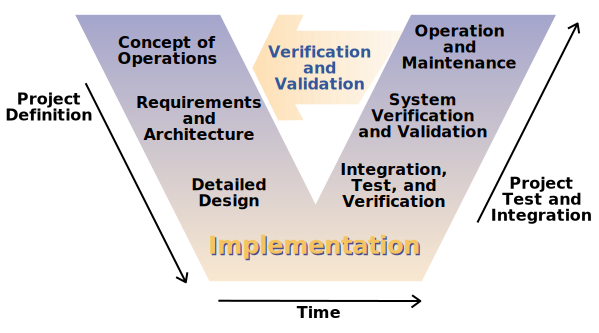
\includegraphics[height=70mm]{Figures/VandV}
  \end{center}
  \caption{Verification and Validation Diagram for a Systems
    Engineering Life Cycle \cite{vandv}}
\end{figure}
The left side of the V\&V diagram highlights all of the required
design while the right side details the build. For undergraduate engineering courses the Design, Build, Test (DBT) framework is often used and has been used at the University of South Alabama for many years with much success. The systems engineering life cycle is a more detailed version of the DBT framework. The systems engineering life cycle is used in many industries including aerospace, automotive, and software development. At the undergraduate level the following steps are used for a standard 16 week curriculum.

\begin{enumerate}[itemsep=-5pt]
  \item {\bf Week 1:} {\it Title Page and Group Development} - Students are given an explanation of the project scope, rubric are asked to split into teams to create a title page and team name. In aircraft design the project is to design, build and test a radio controlled aircraft. In spacecraft design the project is to design, build and test a model rocket. In Instrumentation and Experimental Methods the project is to design, build and test a data acquisition system with at least 3 electrical components not counting the CPU, flash memory, or power supply. This also includes mechanical subsystems so that students practice both hardware and software integration. The teams are typically 1-3 students each depending on class size.
  \item {\bf Week 2:} {\it Concept of Operations (ConOps)} - Students are given an explanation of the ConOps and asked to create a ConOps for their project as well as include a list of requirements which is based on the project scope given by the instructor as well as any additional requirements the students feel are necessary.
  \item {\bf Week 3:} {\it Conceptual Design} - Students are asked to create a hand sketch of their project as well as a brief list of materials they will need to complete the project. This also includes a list of subsystems and components that will be needed to complete the project which requires the students to create a Block Definition Diagram (BDD) as well as an Internal Block Diagram (IBD).
  \item {\bf Week 4:} {\it Preliminary Design} - For the preliminary design phase the task is different depending on the course. In Aircraft Design the students are asked to perform a feasibility analysis and look at overall wingspan, chord and an initial weight estimate. In spacecraft design the students need to look at creating rockets in OpenRockt and perform a preliminary analysis of the rocket's stability. In Instrumentation and Experimental Methods the students need to create more detailed BDDs and IBDs for the mechanical, electrical and software subsystems as well as create an initial interface diagram (ID) for the project.
  \item {\bf Weeks 5-7:} {\it Detailed Design} - The detailed design phase is broken into 3 separate weeks. For aircraft design the students are asked to design the aerodynamic surfaces (wing and tail), the airframe and finally the propulsion system. For spacecraft design the students need to design the structure, propulsion system and perform a detailed trajectory analyis of their rocket. For Instrumentation and Experimental Methods the students need to design the mechanical, electrical and software subsystems creating schematics, wiring diagrams and a list of all software needed to run their system. For every course the students also need to create a detailed bill of materials with prices, weights and links. At this point the system is ready to be built.
  \item {\bf Week 8:} {\it Build Plan, Purchase materials + Break} - In the Fall semester, Fall break typically lands on Week 8 and in the spring Week 8 is typically spring break. As such Students are asked to create a build plan which is not something to be turned in but just something helpful to keep students on track as well as purchase all parts necessary while they are on holiday. If parts are purchased the Friday before break that typically gives the retail stores over 5 business days or 9 calendar days to ship the parts to the students before they return to class. This way students can immediately start building and testing during Week 9 when they return
  \item {\bf Weeks 9-11:} {\it Build and Subsystem Testing} - The build process includes building everything component by component and testing each subsystem as it is built. This is important to ensure that each subsystem works properly independently before integrating everything together. For aircraft design the students will first build the airframe, then the propulsion system and finally the payload which is typically just a datalogger that measures acceleration and GPS location. For spacecraft design the students will first build the structure, then the propulsion system and finally the payload which for spacecraft design is a datalogger that measures acceleration and pressure. For Instrumentation and Experimental Methods the students will test each electrical component one by one and test the software for that specific component. The mechanical system is something to be built and integrated in Week 12.
  \item {\bf Weeks 12-13:} {\it System Integration and Testing} - The integration process includes integrating all subsystems together and testing the entire system as a whole. For aircraft design the students will integrate the airframe, propulsion system and payload and perform a ground test to ensure everything works properly. For spacecraft design the students will integrate the structure and payload and perform a series of tests to ensure everything works properly. This includes a shock cord test, a drop test, a datalogger test, a motor integration test and a nose cone test. For Instrumentation and Experimental Methods the students will integrate all electrical and software subsystems and perform a test without the mechanical subsystem in the way.
  \item {\bf Weeks 14-16:} {\it Final Testing and Validation} - The final testing and validation phase includes performing the final test of the entire system. For aircraft design the students will perform a flight test of their aircraft and recover the data from the datalogger. For spacecraft design the students will perform a launch of their rocket and recover the data from the datalogger. For Instrumentation and Experimental Methods the students will integrate the mechanical subsystem and perform a final test of the entire system. Note that 3 weeks are alloted for this phase to account for weather delays, part delays and any other unforeseen issues that may arise. Many times especially in aircraft design the system fails sometimes catastrophically as in a crash and the students need time to rebuild and retest before the final presentation.
  \item {\bf Week 17:} {\it Final Report and Presentation} - Although a semester is exactly 16 weeks, the final report and presentation is typically due the first week of finals which ends up being Week 17. The final report includes a summary of the entire project including all diagrams, analyses, test results and conclusions. The final presentation is a 10-15 minute presentation to the class and any invited guests which summarizes the entire project. Note that the final report and presentation is typically worth 30-40\% of the overall grade so it is important that students take this seriously and put in their best effort. Furthermore, there are no exams or quizzes in these project based courses so the final report and presentation is the only way to demonstrate what the students have learned throughout the semester. This gives the students ownership of the project and motivates them to do their best work.
\end{enumerate}

\subsection{Block Definition Diagrams (BDDs)}

\subsection{Internal Block Diagrams (IBDs)}

\subsection{Interface Diagrams} 

Interface Diagrams (IDs) are important for many reasons. The biggest
reason that these diagrams are created and maintained is to create
visibility within each subsystem team in a systems engineering7
project. It is crucial that each member working on a project has a
general or even an expert understanding of each subsystem. During the
design process, it is important that each function of each subsystem’s
component is documented so that the current design selection is
recorded and so each of the member’s is familiar with each subsystem
and all of its functionalities. The following image is the ID for the
attitude control and maneuver electronics subsystem on the Gemini Spacecraft.  
\begin{figure}[H]
  \begin{center}
  \includegraphics[height=70mm]{Figures/ACME_ID}
  \end{center}
  \caption{ACME Interface Diagram from the Gemini Spacecraft\cite{qp10}}
\end{figure}
This is an example of an interface diagram for a small subsystem of a
large systems engineering project. The spacecraft requires several
subsystems to work together in the design and fabrication
process. Each of these subsystems has their own ID as well. This is a
good example to introduce you to what these diagrams are. The left
side of the image is the digital computer  which has an accumulator
which flows to the ladder logic block. From the ladder logic flows
several functions into both the attitude control and maneuver
electronics and attitude display blocks. This ID is simple since there
are only four components with many functions, however, many
complicated systems can have extremely complex diagrams. The Figure
below is an example of an ID for an entire spacecraft with all of the 
subsystems included in the diagram.
\begin{figure}[H]
  \begin{center}
  \includegraphics[height=70mm]{Figures/NewHorizons_ID}
  \end{center}
  \caption{New Horizons Interface Diagram\cite{qp11}}
\end{figure}
\subsection{Activity Diagrams}
Activity diagrams are similar to a flowchart.  It is a tool for
representing the sequence of Actions that describe the behavior of a
Block or other structural element. The sequence of execution is
defined using Control Flows. The Actions in an activity diagram can
contain Input and Output Pins which act as buffers for items that flow
from one action to another. Anything that can be produced, consumed,
or conveyed by the system is considered to be an item. Physical
materials, energy, power, data, and information are examples of items\cite{qp12}.

Activity diagrams are useful for engineering modeling.  It conveys
high-level functions and operations to the user. The main purpose of
an activity diagram is to draw the activity or action flow of a
system. Next, it is used to describe the sequence from one activity to
another. Finally, an activity diagram describes the parallel,
branched, and concurrent flow of the system \cite{qp13}.

Activity diagrams are important to the design process because they
maintain coherence throughout the project. If a system is composed of
multiple, intertwining subsystems, a person can simply follow the
activity diagrams to understand how each component and subsystem
interacts with one another. Activity diagrams also describe the data
flow of a system and when or where that data is created, converted or
used. Overall, activity diagrams are the roadmap of a system and
describe the intricacies of how it operates.  

As stated previously, activity diagrams denote how components and
subsystems interact with each other. This is accomplished through the
use of swimlanes which keep separate the individual activities and
object flows of a component or subsystem. Swimlanes are the boxes
which contain activities, however control and object flows can
traverse swimlanes. Activities which have inputs and outputs will also
have a pin attached to them. This small rectangular box denotes when
matter, energy or data flow is created or destroyed.  

The main purpose of activity diagrams is to show the control flow of
the system. This control flow refers to the execution path of an
activity. Control flow is indicated by control nodes for which there
are seven different kinds. Each control node is described in the table below.
\begin{table}[H]
  \begin{center}
    \begin{tabular}{c|p{7cm}|c}
      \hline
      Control Node & Description & Appearance \\
      \hline
      \hline
      Initial Node & The beginning of an activity sequence & Black
      circle \\
      \hline
      Activity Final Node & The end of an activity sequence & Black
      circle within a circle \\
      \hline
      Flow Final Node & The end of one branch of an activity sequence,
      but not the entire activity diagram. & Circle with an 'X' in it
      \\
      \hline
      Decision Node & The splitting point of an activity flow based on
      the outcome of a boolean operator such as ‘isCommandValid
      ==True’. One flow in comes in, while two flows come out as
      branching paths. & Diamond \\
      \hline
      Merge Node & The merging point of two activity paths. Two flows
      come in, while one flow comes out. & Diamond \\
      \hline
      Fork Node & The distribution of an activity flow into multiple
      pathways. When one object or control token comes in, it is
      duplicated into multiple paths. & Black bar \\
      \hline
      Join Node & The joining point of multiple synchronized
      concurrent flows. Two concurrent flows come in, while one flow
      comes out. & Black bar \\
      \hline
      \hline
    \end{tabular}
  \end{center}
\end{table}
